% === [ Appendices ] ===========================================================

\appendix
\setcounter{secnumdepth}{0}
\section{Appendices}
\setcounter{secnumdepth}{3}
\renewcommand{\thesubsection}{\Alph{subsection}}

% --- [ Project Initiation Document ] ------------------------------------------

\subsection{Project Initiation Document}


\includepdf[pages=-]{appendices/PID.pdf}

% --- [ Certificate of Ethics Review ] -----------------------------------------

\subsection{Certificate of Ethics Review}

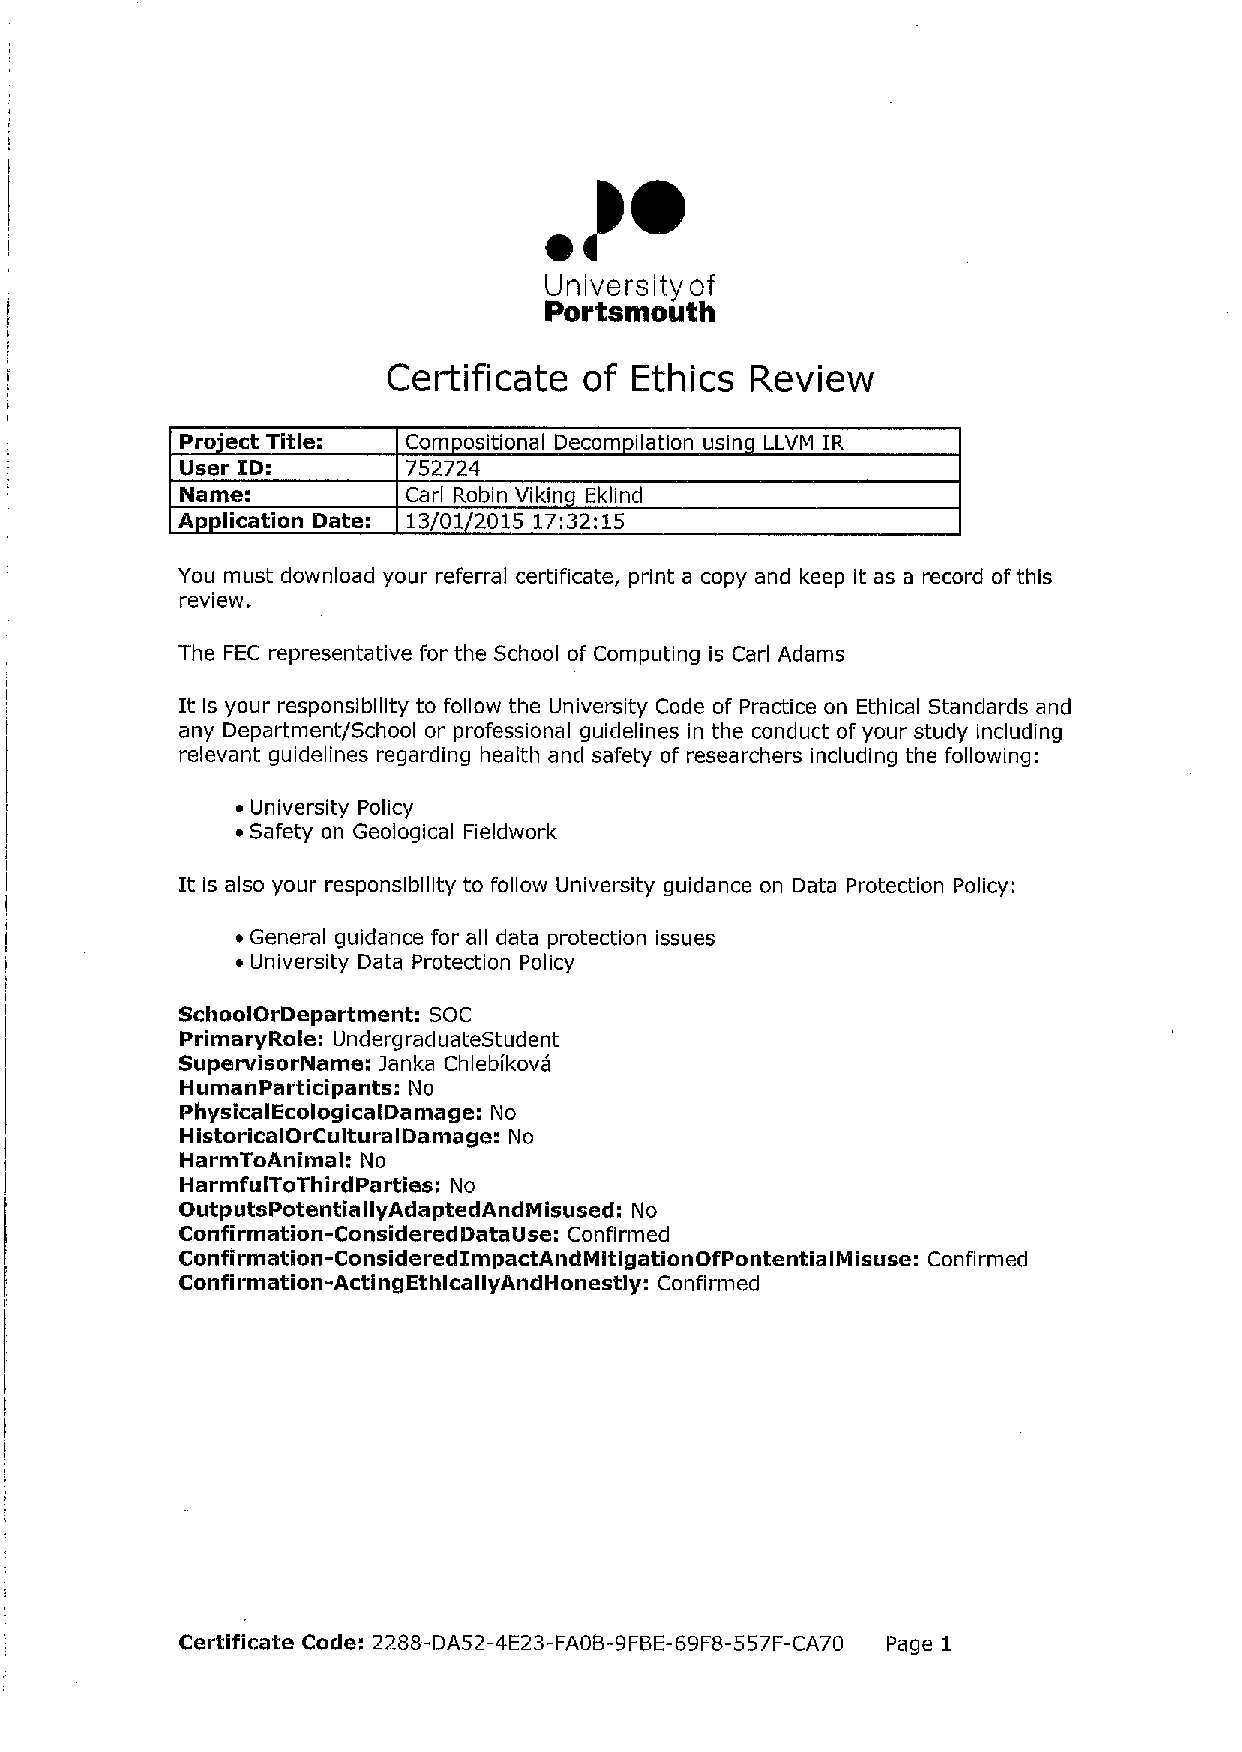
\includepdf[pages=-]{appendices/ethics_review.pdf}

% --- [ Gantt Chart ] ----------------------------------------------------------

\subsection{Initial and Final Gantt Charts}

\begin{figure}[htbp]
	\begin{center}
		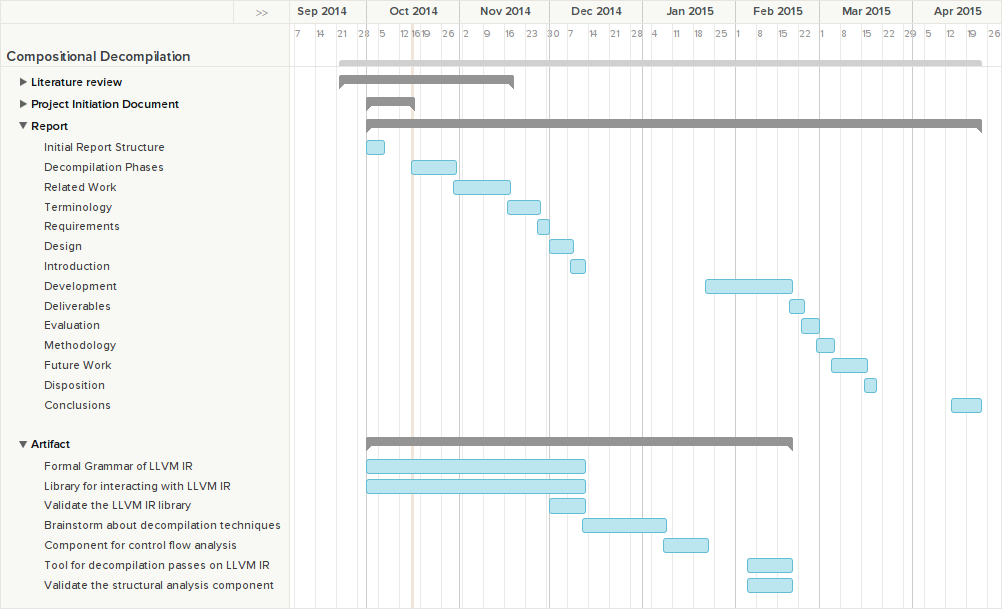
\includegraphics[angle=270, width=0.9\textwidth]{appendices/gantt_initial.png}
		\caption{Initial Gantt chart.}
	\end{center}
\end{figure}

% TODO: Add final Gantt chart.

\pagebreak

% --- [ The REIL Instruction Set ] ---------------------------------------------

\subsection{The REIL Instruction Set}
\label{app:reil_instructions}

\lstinputlisting[language=reil, style=nasm, caption={A full definition of the REIL instruction set. \label{lst:reil_instructions}}]{appendices/reil_instruction_set.asm}

\pagebreak

% --- [ Patch for Unnamed Basic Blocks of LLVM ] -------------------------------

\subsection{Patch for Unnamed Basic Blocks of LLVM}
\label{app:unnamed_patch}

The following patch ensures that the assembly printer of LLVM 3.6.0 always prints the generated names of unnamed basic blocks.

\lstinputlisting[language=diff, style=diff, caption={Always print the generated names of unnamed basic blocks. \label{lst:unnamed_patch}}]{appendices/unnamed.patch}
